% Clase del documento
\documentclass[12pt,twoside,titlepage]{report}





%%%%%%%%%%%%%%%%%%%%%%% Paquetes %%%%%%%%%%%%%%%%%%%%%%%

\usepackage[a4paper,bindingoffset=3mm,bottom=35mm]{geometry}


% Usad \usepackage[dvips]{graphicx} o \usepackage[pdftex]{graphicx} (no ambos)
%\usepackage[dvips]{graphicx} %%% para LaTeX. Las figuras deben estar en formato eps

\usepackage[colorlinks=true,pdftex]{hyperref}   %%% Opcional. Para incluir marcadores y enlaces en el pdf
\usepackage[pdftex]{graphicx}  %%% para pdflatex. Las figuras pueden estar en pdf, jpg, svg y otros formatos


\usepackage[spanish]{babel}

%\usepackage[latin1]{inputenc} % Usad en WinEdt/MikTex
\usepackage[utf8]{inputenc} % Usad en overleaf

%\usepackage[T1]{fontenc}


% Algunos paquetes útiles

\usepackage{amsmath,amssymb}
\usepackage{hyperref}
\usepackage{xcolor}
\usepackage{afterpage}
%\usepackage{paralist}
\usepackage{array}
\usepackage{enumerate}
\usepackage{paralist}
\usepackage{enumitem}
\usepackage{float}
\usepackage{setspace}
\usepackage{listings}
\usepackage{algorithm}
\usepackage{algorithmic}
\usepackage{fancyhdr}
\usepackage{rotating}
\usepackage{multirow}

% Otros paquetes

\usepackage{quotchap}
\usepackage{lipsum}

%%%%%%%%%%%%%%%%%%%%%%%%%%%%%%%%%%%%%%%%%%%%%%%%%%%%%%%%






%%%%%%%%%%%%%%%%%%%%%%% Definiciones básicas %%%%%%%%%%%%%%%%%%%%%%%

\newcommand{\nombreautor}{Gonzalo Ortega Carpintero}
\newcommand{\nombretutor}{Alberto Fernández Gil}
\newcommand{\nombretutorcsic}{Pablo Jercog}
\newcommand{\titulotrabajo}{Métodos de aprendizaje automático para la clasificación de comportamientos estereotipados}
\newcommand{\escuela}{Escuela Técnica Superior\\de Ingeniería Informática}
\newcommand{\escuelalargo}{Escuela Técnica Superior de Ingeniería Informática}
\newcommand{\universidad}{Universidad Rey Juan Carlos}
\newcommand{\fecha}{Fecha}
\newcommand{\grado}{Grado en Ingeniería del Software}
\newcommand{\curso}{Curso 2023-2024}
\newcommand{\logoUniversidad}{figures/logoURJC.pdf}

%%%%%%%%%%%%%%%%%%%%%%%%%%%%%%%%%%%%%%%%%%%%%%%%%%%%%%%%%%%%%%%%%%%%






%%%%%%%%%%%%%%%%%%%%%%%%% Otras definiciones %%%%%%%%%%%%%%%%%%%%%%%%%%

% Definiciones de colores (para hidelinks)
\definecolor{BlueLink}{rgb}{0.165,0.322,0.745}
\definecolor{PinkLink}{rgb}{0.8,0.22,0.5}
\definecolor{gray}{rgb}{0.6,0.6,0.6}


% Enlaces
\hypersetup{hidelinks,pageanchor=true,colorlinks,citecolor=PinkLink,urlcolor=black,linkcolor=BlueLink}


\newcommand\blankpage{%
    \newpage
    \null
    \thispagestyle{empty}%
    %\addtocounter{page}{-1}%
    \newpage}


% Texto referencias
\addto{\captionsspanish}{\renewcommand{\bibname}{Bibliografía}}

% Texto Índice de tablas
\addto\captionsspanish{
\def\tablename{Tabla}
\def\listtablename{\'{I}ndice de tablas}
}


\floatname{algorithm}{Algoritmo}

\newfloat{algorithm}{t}{lop}

%% Etiquetas de comentarios (tutor/alumno)
\newif\ifdraft
\drafttrue
\usepackage{subcaption}
\newcommand{\nb}[2]{
	{
		{\color{black}{
				\small\fbox{\bfseries\sffamily\scriptsize#1}
				{\sffamily\small$\triangleright~${\it\sffamily\small #2}$~\triangleleft$}
	}}}
}

\ifdraft
\newcommand\tutor[1]{\nb{Tutor}{\color{red}#1}}
\newcommand\alumno[1]{\nb{Alumno}{\color{blue}#1}}
\newcommand\cotutor[1]{\nb{Co-tutor}{\color{green}#1}}
\newcommand{\fixme}[1]{{\textcolor{red}{[FIXME] #1}}\xspace}
\newcommand{\cn}{{\color{violet}[citation required]}}

\else
%\usepackage[disable]{todonotes}
\newcommand\tutor[1]{}
\newcommand\alumno[1]{}
\newcommand\cotutor[1]{}
\newcommand{\fixme}[1]{}
\newcommand{\cn}{}

\fi






%\newenvironment{pseudocodigo}[1][htb]
%  {\renewcommand{\algorithmcfname}{Pseudocódig}% Update algorithm name
%   \begin{algorithm}[#1]%
%  }{\end{algorithm}}
  
%%%%%%%%%%%%%%%%%%%%%%%%%%%%%%%%%%%%%%%%%%%%%%%%%%%%%%%%%%%%%%%%%%%%





%%%%%%%%%%%%%%%%%%%%%%% Estilo de código (en Python) %%%%%%%%%%%%%%%%%%%%%%%

\definecolor{bg}{rgb}{0.95,0.95,0.95}
\definecolor{mydeepteal}{rgb}{0.16,0.22,0.23}
\definecolor{myteal}{rgb}{0.31,0.44,0.46}
\definecolor{mymediumteal}{rgb}{0.41,0.58,0.60}

\DeclareFixedFont{\ttb}{T1}{txtt}{bx}{n}{12} % for bold
\DeclareFixedFont{\ttm}{T1}{txtt}{m}{n}{12}  % for normal


%\newcommand*{\FormatDigit}[1]{\textcolor{mydeepteal}{#1}}
\newcommand*{\FormatDigit}[1]{\textcolor{black}{#1}}

% Python style for highlighting
\newcommand\mypythonstyle{\lstset{
language=Python,
basicstyle=\ttfamily\small,
%basicstyle=\linespread{1.0}\footnotesize\ttm,
otherkeywords={self},             % Add keywords here
keywordstyle=\bfseries\ttfamily\color{myteal},
%keywordstyle=\ttb\color{myteal},
commentstyle=\itshape\color{myteal},
stringstyle=\color{mydeepteal},
emph={MyClass,__init__},          % Custom highlighting
emphstyle=\ttb\color{mydeepteal},    % Custom highlighting style
% Any extra options here
showstringspaces=false,            %
backgroundcolor=\color{bg},
rulecolor = \color{bg},
%identifierstyle=\color{deepgreen},
breaklines=true,
numbers=left,
numbersep=5pt,
numberstyle=\tiny,
tabsize=4,
xleftmargin=1em,
frame = single,
framesep = 3pt,
framextopmargin=0pt,
framexbottommargin=0pt,
framexleftmargin=0pt,
framexrightmargin=0pt,
fontadjust=true,
basewidth=0.55em, % compactness of code
upquote=true,
}}

% Python environment
\lstnewenvironment{mypython}[1][]
{
\mypythonstyle
\lstset{#1}
}
{}

\newcommand\mypythonstylenormalinline{\lstset{
language=Python,
basicstyle=\ttfamily\normalsize,
%basicstyle=\linespread{1.0}\footnotesize\ttm,
otherkeywords={self},            % Add keywords here
keywordstyle=\bfseries\ttfamily\color{myteal},
%keywordstyle=\ttb\color{myteal},
commentstyle=\itshape\color{mymediumteal},
stringstyle=\color{mydeepteal},
emph={MyClass,__init__},          % Custom highlighting
emphstyle=\ttb\color{mydeepteal},    % Custom highlighting style
% Any extra options here
showstringspaces=false,            %
backgroundcolor=\color{bg},
rulecolor = \color{bg},
%identifierstyle=\color{deepgreen},
breaklines=false,
numbers=left,
numbersep=5pt,
numberstyle=\tiny,
tabsize=4,
xleftmargin=0em,
frame = single,
framesep = 3pt,
framextopmargin=0pt,
framexbottommargin=0pt,
framexleftmargin=0pt,
framexrightmargin=0pt,
fontadjust=true,
%basewidth=0.55em, % compactness of code
upquote=true,
}}

\newcommand\mypythoninline[1]{{\mypythonstylenormalinline\lstinline!#1!}}

%%%%%%%%%%%%%%%%%%%%%%%%%%%%%%%%%%%%%%%%%%%%%%%%%%%%%%%%%%%%%%%%%%%%%%%%%%%%%%




%%%%%%%%%%%%%%%%%%%%%%%%%%%% Comandos definidos por el autor 

\newcommand{\transpuesta}{\mbox{\tiny $\mathsf{T}$}}








%%%%%%%%%%%%%%%%%%%%%%%%%%%%%%%%%%%%%%%%%%%%%%%%%%%%%%%%%%%%%%%%%%%%%%%
%                           Inicio del documento                       
%%%%%%%%%%%%%%%%%%%%%%%%%%%%%%%%%%%%%%%%%%%%%%%%%%%%%%%%%%%%%%%%%%%%%%%


\begin{document}

\pagestyle{plain}




%%%%%%%%%%%%%%%%%%%%%%%%%%%%%%%%%%%% Portada %%%%%%%%%%%%%%%%%%%%%%%%%%%%%%%%%%

%\pagenumbering{gobble}
%\pagenumbering{arabic}

% Universidad, Facultad
\begin{titlepage}
\selectlanguage{spanish}


% logo
\begin{center}
    \includegraphics[scale=0.7]{\logoUniversidad}
\end{center}

\bigskip

\begin{center}
\begin{LARGE}
\escuela \\
\end{LARGE}
\end{center}

\bigskip
\bigskip

% Grado
\begin{center}
\begin{large}
\textbf{\grado}\\
\end{large}
\end{center}

% Curso
\begin{center}
\begin{large}
\textbf{\curso}\\
\end{large}
\end{center}

\bigskip

\textbf{\begin{center}
\begin{large}
\textbf{Trabajo Fin de Grado}
\end{large}
\end{center}}

\bigskip
\bigskip
\bigskip

% Nombre del TFG
\begin{center}
\textbf{\begin{large}
\MakeUppercase{\titulotrabajo}\\
\end{large}}
\end{center}

% Nombre del autor
\vspace{\fill}
\begin{center}
\textbf{Autor: \nombreautor}\\ \smallskip
% Tutores
\textbf{Tutor URJC: \nombretutor}\\ \smallskip
\textbf{Tutor CSIC: \nombretutorcsic}\\
% Añadir segundo tutor si hubiera


\bigskip

% Fecha
%\textbf{\fecha}\\
\end{center}
\end{titlepage}


%%%%%%%%%%%%%%%%%%%%%%%% Opcional %%%%%%%%%%%%%%%%%%%%%%
%\blankpage

%\thispagestyle{empty}
%\begin{center}

% Nombre del trabajo
%\textbf{\begin{large}
%\MakeUppercase{\titulotrabajo}\\*
%\end{large}}
%\vspace*{0.2cm}
%\vspace{5cm}

% Nombre del autor y del tutor
%\large Autor: \nombreautor \\* \medskip
%\large Tutor: \nombretutor \\*

%\vfill

% Escuela, universidad y fecha
%\escuelalargo \\ \smallskip
%\universidad \\
%\vspace{1cm}
%\fecha \\

%\clearpage

%\end{center}
%%%%%%%%%%%%%%%%%%%%%%%%%%%%%%%%%%%%%%%%%%%%%%%%%%%%%%%%

\hypersetup{pageanchor=true}

\normalsize
\afterpage{\blankpage} % Se deben añadir página en blanco para que lo capítulos de la memoria o estas secciones introductorias empiecen en páginas impares

%%%%%%%%%%%%%%%%%%%%%%%%%%%%%%%%%%%%%%%%%%%%%%%%%%%%%%%%%%%%%%%%%%%%%%%%%%%%%%%


% Estilo de párrafo de los capítulos
\setlength{\parskip}{0.75em}
\renewcommand{\baselinestretch}{1.25}
% Interlineado simple
\spacing{1}

\pagenumbering{Roman}
\setcounter{page}{2}


%%%%%%%%%%%%%%%%%%%%%%%%% Agradecimientos o dedicatoria %%%%%%%%%%%%%%%%%%%%%%%%%%%

\chapter*{Agradecimientos}
A Paula Peixoto Moledo por guiarme en todo el proceso de lectura, desarrollo y redacción de este trabajo y a Jesús González Gironda por mostrarme la oportunidad de realizar este trabajo en el CSIC.
\afterpage{\blankpage}

%%%%%%%%%%%%%%%%%%%%%%%%%%%%%%%%%%%%%%%%%%%%%%%%%%%%%%%%%%%%%%%%%%%%%%%%%%%%%%%%%%%



%%%%%%%%%%%%%%%%%%%%%%%%%%%%%%%%%%%% Resumen %%%%%%%%%%%%%%%%%%%%%%%%%%%%%%%%%%%%%%

\chapter*{Resumen}
A lo largo de la historia, en ciencia en general y en Neurociencia de sistemas en particular, se han realizado todo tipo de experimentos en los cuales los experimentadores tenían que llevar un control manual del proceso, realizando mediciones limitadas sujetas a la interpretación y sesgo de cada experimentador, que necesitaban ser analizadas individualmente. Con el reciente auge de los métodos de aprendizaje automático, ahora es posible recopilar y analizar muchos más datos con un mismo presupuesto, utilizando diversas técnicas para analizar y obtener resultados de los experimentos de forma automática.

Este trabajo se enfoca en distinguir de forma automática los diferentes tipos de comportamientos que realiza un animal en su caja hábitat a lo largo de una sesión de video. Además, busca diferenciar animales control de aquellos que están bajo los efectos de un bloqueador de NMDA. Para ello, primero se realiza una introducción teórica a algoritmos de aprendizaje no supervisado: PCA, agrupación por k-medias, agrupación aglomerada, y agrupación por afinidad; y a algoritmos de aprendizaje supervisado: redes neuronales secuenciales y convolucionales. Posteriormente, se aplican estos algoritmos a datos de la postura corporal de animales a lo largo de sesiones de video procesadas con DeepLabCut, una herramienta de código abierto basada en el aprendizaje profundo, diseñada para rastrear el comportamiento animal con alta precisión.


\mbox{} \bigskip

\noindent \textbf{Palabras clave}:
\begin{compactitem}
    \item Neurociencia de sistemas
    \item Aprendizaje automático
    \item PCA
    \item k-medias
    \item Agrupación aglomerativa
    \item Agrupación por afinidad
    \item Red neuronal secuencial
    \item Red neuronal convolucional
    \item DeepCutLab
    \item Python
\end{compactitem}
\afterpage{\blankpage}

%%%%%%%%%%%%%%%%%%%%%%%%%%%%%%%%%%%%%%%%%%%%%%%%%%%%%%%%%%%%%%%%%%%%%%%%%%%%%%%%%%%



%%%%%%%%%%%%%%%%%%%%%%%%%%%%%%%%%%%% Índices %%%%%%%%%%%%%%%%%%%%%%%%%%%%%%%%%%%%

% Estilo de párrafo de los Índices
\setlength{\parskip}{1pt}
\renewcommand{\baselinestretch}{1}
\renewcommand{\contentsname}{Índice de contenidos}


% Índice de contenidos
\tableofcontents
\afterpage{\blankpage}

% Índice de tablas (OPCIONAL)
\listoftables
\afterpage{\blankpage}
\addcontentsline{toc}{chapter}{\noindent \listtablename}

% Índice de figuras (OPCIONAL)
\listoffigures
\afterpage{\blankpage}
\addcontentsline{toc}{chapter}{\listfigurename}

% Índice de códigos/algoritmos (OPCIONAL).   El término "Códigos" se puede cambiar por "Métodos", "Funciones", "Algoritmos", etc.
\renewcommand\lstlistlistingname{Códigos}
\renewcommand\lstlistingname{Código}
\renewcommand\lstlistlistingname{Índice de códigos}

\lstlistoflistings
\afterpage{\blankpage}
\addcontentsline{toc}{chapter}{\lstlistlistingname}


% En este documento (de momento) no se ha considerado incluir un índice de algoritmos/pseudocódigos, como el que aparece en \ref{AdditionalLouvain}

%%%%%%%%%%%%%%%%%%%%%%%%%%%%%%%%%%%%%%%%%%%%%%%%%%%%%%%%%%%%%%%%%%%%%%%%%%%%%%%%%%%





%%%%%%%%%%%%%%%%%%%%%%% Cabeceras y pies de página (Opcional) %%%%%%%%%%%%%%%%%%%%%%%

%\setlength{\headheight}{15.2pt}
\pagestyle{fancy}


\renewcommand{\chaptermark}[1]{\markboth{Capítulo \thechapter.\ #1}{}}

\pagestyle{fancy}
\fancyhf{}
\fancyhead[LO]{\leftmark}
\fancyhead[RO]{}
\fancyhead[RE]{\nouppercase\rightmark}
\fancyhead[LE]{}
\fancyfoot[C]{\thepage}

%%%%%%%%%%%%%%%%%%%%%%%%%%%%%%%%%%%%%%%%%%%%%%%%%%%%%%%%%%%%%%%%%%%%%%%%%%%%%%%%%%%%






%%%%%%%%%%%%%%%%%%%%%%%%%%%%%% Capítulos de la memoria %%%%%%%%%%%%%%%%%%%%%%%%%%%%%

% Estilo resto de páginas
\pagestyle{fancy}
% Estilo de párrafo de los capítulos
\setlength{\parskip}{0.75em}
\renewcommand{\baselinestretch}{1.25}
% Interlineado simple
\spacing{1}
% Numeración contenido


%%%%%%%%%%%%%%%%%%%%%%%%%%%%%%%%%%%%%%%%%%%%%%%%%%%%%%%%%%%%%%%%%%%%%%%%%%

\chapter{Introducción}
Este documento recoge el Trabajo de Fin de Grado (TFG) de Gonzalo Ortega Carpintero, incluido en el itinerario del grado en Ingeniería del \textit{Software} de la Universidad Rey Juan Carlos.

En este primer capítulo se presenta la motivación que ha dado lugar a la idea y desarrollo de este TFG en la Sección \ref{sec:motivacion}. En la Sección \ref{sec:objetivos} se introduce el objetivo principal del trabajo y se enumeran los objetivos parciales que se han propuesto para conseguirlo. En la Sección \ref{sec:metodología} se hace un repaso a la metodología seguida para realizar el trabajo y finalmente, en la Sección \ref{sec:herramientas} se introducen las herramientas y bibliotecas que se han utilizado.

\section{Motivación} \label{sec:motivacion}

La Neurociencia de sistemas es (DEFINICIÓN). Para el estudio del funcionamiento del cerebro pueden utilizarse multitud de técnicas diferentes, pero para evitar la intrusión en el sujeto de estudio de muchas de ellas, muchos experimentos e investigaciones se basan en el estudio del comportamiento. Es la etología la encargada de este tipo de estudio en animales y en la cual, históricamente, la categorización de comportamientos dependía fuertemente de la observación manual. Eso ha conllevado siempre una excesiva cantidad de tiempo y las desventajas de los posibles errores de percepción humanos, limitando la cantidad y la calidad de los análisis a realizar.

Gracias a los recientes avances en algoritmos de aprendizaje automático, hoy en día es posible computar multitud de datos de forma simultánea, agilizando y automatizando análisis como el ilustrado previamente.

Este Trabajo de Fin de Grado se ha realizado a lo largo de una estancia de prácticas académicas en el Jercog's Team, un equipo de investigación perteneciente al Instituto Cajal, instituto de Neurociencia del Consejo Superior de Investigaciones Científicas. El equipo está centrado en el estudio de la memoria mediante experimentos con ratones, y uno de sus proyectos abiertos consistía en poder elaborar una herramienta para clasificar automáticamente los comportamientos estereotipados de los ratones. Estos son comportamientos cortos, repetitivos y con cierta tendencia a generar patrones, tales como rascarse, caminar en círculos o levantarse a dos patas, ejecutados sin ninguna finalidad, y usualmente inducidos por estar en entornos cerrados y artificiales.

Para la ejecución de uno de sus últimos experimentos utilizan ratones tratados con anticuerpos bloqueadores de NMDA (\textit{N-Metil-D-aspartato}), restringiendo la capacidad de los ratones para almacenar memoria a largo plazo. En las sesiones de experimentación los ratones tratados ejercen las mismas tareas que ratones control, tratados con un suero placebo, y en las grabaciones hay ratones de ambos tipos. A ojo de un experimentador, es complejo determinar a ciegas si un ratón está bajo los efectos de NMDA o es control, por lo que es interesante la posibililidad de contar con una herramienta que sea capaz de distinguir unos de otros a partir de los videos de las sesiones.

Durante la estancia se han valorado multitud de técnicas de análisis y procesado de datos, haciendo hincapié en métodos de aprendizaje automático para tratar de completar el proyecto gracias a los últimos avances en computación.

\section{Objetivos} \label{sec:objetivos}
El objetivo de este trabajo es distinguir de forma automática, mediante la clasificación de los comportamientos o de forma directa, si un animal está bajo los efectos de un bloqueador de MDMA.

\subsection{Hipótesis}
Para contrastar nuestro objetivo hemos planteado la siguiente hipótesis:

\textit{Dados los datos de posición de una serie de puntos de un ratón en su caja a lo largo de una sesión de video, mediante técnicas de aprendizaje automático, es posible diferenciar diferentes comportamientos del ratón, e identificar si está bajo los efectos de un bloqueador de NMDA.}

\subsection{Objetivos parciales}
Con el fin de desglosar el objetivo principal, y de poder corroborar o refutar nuestra hipótesis, hemos planteado varios objetivos parciales.

\begin{itemize}
    \item Realizar una introducción a técnicas de aprendizaje automático aplicables al procesado de datos en el análisis de experimentos con animales.
    \item Preparar y preprocesar datos provenientes de archivos de video para su posterior análisis.
    \item Aplicar algoritmos de agrupación para separar fragmentos de video y clasificarlos en función del comportamiento que esté realizando el animal.
    \item Aplicar algoritmos no supervisados para distinguir animales control de animales tratados.
    \item Aplicar algoritmos supervisados para distinguir animales control de animales tratados.
\end{itemize}


\section{Metodología} \label{sec:metodología}

El trabajo se divide en dos capítulos principales, en el Capítulo \ref{chap:fundamentos-teoricos} abordaremos el estudio teórico de ciertos algoritmos de agrupamiento, reducción de dimensionalidad y de clasificación supervisada. Todo ello desde un punto de vista teórico con ejemplos fáciles de visualizar para ayudar al lector a comprender en profundidad los métodos.

En el Capítulo \ref{chap:analisis-y-experimentacion}, desarrollaremos paso a paso el análisis real ejercido durante la estancia en el Instituto Cajal. El principal objetivo durante estos meses ha sido buscar la mejor forma de, dados una serie de videos de ratones en su caja, detectar automáticamente diferentes tipos de comportamientos. El fin último del proyecto es estudiar la posibilidad de clasificar dos grupos de animales, control y medicados, basándose en los comportamientos estereotipados.

\section{Bibliotecas y herramientas utilizadas} \label{sec:herramientas}

\subsection*{DeepLabCut}
DeepLabCut \cite{deeplabcut} es una herramienta para la estimación 2D y 3D sin marcadores mediante el uso de redes neuronales. Es capaz de identificar de rastrear diferentes partes del cuerpo de múltiples especies realizando todo tipo de comportamientos. Esta ha sido la base de todo nuestro trabajo, ya que todos los videos que hemos analizado han sido procesados en primer lugar por DeepLabCut para rastrear las posiciones de múltiples puntos de los animales a lo largo de los videos de las sesiones. Debido a su importancia, damos una explicación más en detalle de su funcionamiento y de como lo hemos utilizado en la sección \ref{sec:DeepLabCut}.

\subsection*{Google Colab}
Google Colab es una herramienta para realizar cuadernos de Jupyter en línea, y poder ejecutarlos en el \textit{backend} de Google. Estos son documentos que intercalan fragmentos de texto con fragmentos de código ejecutable en Python, así como la salida de las distintas ejecuciones. Todo el codigo realizado para este trabajo ha sido realizado en cuadernos de Colab, y puede ser consultado en los siguientes enlaces:

% Colab links
\begin{table}[h]
    \centering
    \begin{tabular}{|c|p{10cm}|}
        \hline
        \textbf{Ejemplos teóricos} & \href{https://colab.research.google.com/drive/
        1qLLQTCFLZcqExN7qyYyRAT1nm7P8NhuK?usp=sharing}{https://colab.research.google.com/drive/ 1qLLQTCFLZcqExN7qyYyRAT1nm7P8NhuK?usp=sharing} \\
        \hline
        \textbf{DeepCutLab} & \href{https://colab.research.google.com/drive/1dFbmUcfW9el50v0RBCkLIItTD6SF7A3x?usp=sharing}{https://colab.research.google.com/drive/
        1dFbmUcfW9el50v0RBCkLIItTD6SF7A3x?usp=sharing} \\
        \hline
        \textbf{Análisis principal} & \href{https://colab.research.google.com/drive/
        1ak2VpDi-zTnV-uEDp-viEkpa8GFDGuBR?usp=sharing}{https://colab.research.google.com/drive/ 1ak2VpDi-zTnV-uEDp-viEkpa8GFDGuBR?usp=sharing} \\
        \hline
    \end{tabular}
    \caption{Enlaces a cuadernos de Google Colab.}
    \label{tab:colab-links}
\end{table}

\subsection*{Scikit-learn}
Scikit-learn \cite{scikit-learn} es una biblioteca de código abierto de Python que contiene numerosas implementaciones de algoritmos de aprendizaje automático. Hemos usado dichas implementaciones tanto como para la explicación teórica de los algoritmos, como para el análisis real de los datos de los animales.

\subsection*{PyTorch}
\cite{pytorch-paper}

\subsection*{pandas}
\texttt{pandas} es una biblioteca de manejo de datos mediante tablas denominadas \texttt{DataFrame}. Todos los datos que hemos cargado para ser analizados los hemos guardado como {DataFrames} para poder tener un fácil acceso a todos ellos y a sus variables pudiendo, además, visualizarlos de una forma sencilla.

\subsection*{NumPy}
NumPy es una de las bibliotecas principales de cálculo científico en Python. Proporciona un objeto de \texttt{array} multidimensional y numerosas funciones estadísticas y algebraicas de mucha utilidad.

\subsection*{matplotlib}
\texttt{matplotlib} es una biblioteca para crear figuras en Python. Todas las figuras de representación de datos que aparecen en este trabajo han sido creadas con \texttt{matplotlib}. El código concreto utilizado para generarlas puede consultarse en los cuadernos de Colab.


%\chapter{Objetivos}
%Objetivos generales y específicos del trabajo.


\section{Primera sección}

En este capítulo se pueden añadir secciones, pero no son obligatorias en capítulos cortos.

\section{Segunda sección}

El objetivo de este documento es proporcionar una plantilla de \LaTeX para TFG. No debe usarse como sustituto de la normativa de TFG aprobada por la ETSII.



\section{Métodos no supervisados}

Los algoritmos de aprendizaje automático no supervisados se utilizan cuando no se conoce la salida esperada. Al algoritmo de aprendizaje se le otorgan los datos de entrada y se le pide extraer información de estos datos. Las principales aplicaciones de estos algoritmos, las cuales vamos a aprovechar, son la agrupación de datos y la reducción de dimensionalidad de las variables de los mismos. Esa última es usada principalmente para poder hacer representaciones de datos multidimensionales, los cuales serian complejos de visualizar de otra forma.

La principal pega que pueden tener estos algoritmos es que, si bien no siempre son capaces de identificar conocimiento dados los datos utilizados, cuando lo obtienen, no siempre es el conocimiento que esperábamos obtener. Póngase el ejemplo de un algoritmo que tratase de agrupar rostros de personas iguales. Al no darle a priori ningún tipo de salida de ejemplo, el algoritmo puede acabar clasificando si los rostros están de frente o de lado, no precisamente lo que esperábamos. Es por ello que estos algoritmos cuentan con diversidad de parámetros para ajustarlos a nuestras necesidades, tratando de realizar la agrupación deseada.

En esta sección vamos a estudiar a fondo tres tipos de algoritmos de agrupación: el agrupamiento por k-medias, la agrupación aglomerada, y la agrupación por afinidad. Además, estudiaremos también el principal algoritmo de reducción de dimensiones, el análisis de componentes principales, PCA, de sus siglas en inglés. Los principales ejemplos y explicaciones de los algoritmos han sido inspirados por los dados en el libro \cite[Introduction to Machine Learning with Python]{machine}.

Para analizar los diferentes métodos hemos utilizado \texttt{scikit-learn} para generar una muestra sintética de datos bidimensionales agrupados en dos lunas.

\begin{mypython}[float={h},caption={Generación de datos sinteticos.}]
    X, y = skl.make_moons(n_samples=200,
                          noise=0.05,
                          random_state=0)
    
    def figure_scatter_data(data, assignment=None):
      fig = plt.figure(figsize=(5, 5))
      ax = fig.add_subplot(111)  
      if assignment is not None:
        ax.scatter(data[:, 0], data[:, 1], c=assignment, cmap='Pastel1')
      else:
        ax.scatter(data[:, 0], data[:, 1], alpha=0.5)

      ax.set_xlabel('X')
      ax.set_ylabel('Y')  

    figure_scatter_data(X)
\end{mypython}

En la tabla \ref{tab:colab-links} está el enlace para poder ejecutar el código en el \textit{backend} de Google.

\begin{figure}[h]
    \centering

    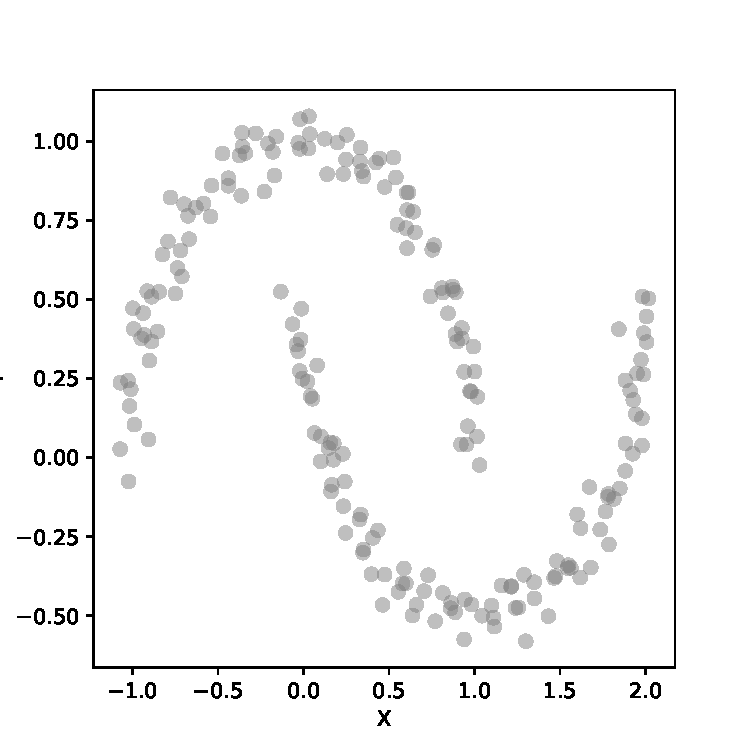
\includegraphics[width=0.5\textwidth]{figures/fake-data.pdf}
    \caption[Datos artificiales]{Datos artificiales en forma de dos lunas para probar los diferentes tipos de agrupaciones.}
    \label{fig:fake-data}

\end{figure}

\subsection{Agrupamiento por K-medias}
El algoritmo de k-medias clasifica los datos separando los datos en $n$ grupos de con la misma varianza.

El algoritmo comienza inicializando aleatoriamente $n$ centroides, siendo $n$ el número de agrupaciones que se le han dicho que realice. Estos centroides serán los centros de las agrupaciones que va a realizar, no tienen por qué pertenecer a los datos, pero sí que están contenidos en su misma dimensión. En cada iteración, el algoritmo asigna a cada punto de los datos el centroide más próximo y luego asigna a cada agrupación un nuevo centroide calculado como la media de los datos que se han asignado a dicha agrupación.

Formalmente, el algoritmo divide un conjunto de $n$ puntos $x$ en $k$ agrupaciones disjuntas $C$, cada una descrita por la media $\mu_j$ de los puntos en la agrupación. Para ello, el algoritmo trata de encontrar los centroides que minimicen

\begin{equation}
  \sum\limits_{i=0}^n \underset{\mu_j \in C}{\operatorname{min}} (|| x_i - \mu_j||^2)
\end{equation}

El algoritmo finaliza cuando una iteración no realice ninguna modificación de las agrupaciones.

\begin{mypython}[float={h},caption={k-medias.}]
    kmeans = KMeans(n_clusters=2, n_init="auto")
kmeans_assigment = kmeans.fit_predict(X)
\end{mypython}

\subsection{Agrupación aglomerada}

\begin{mypython}[float={h},caption={Propagación de afinidad.}]
    agg = AgglomerativeClustering()
    agg_assigment = agg.fit_predict(X)
\end{mypython}

\subsection{Agrupación por afinidad}

El algoritmo de propagación de afinidad crea agrupaciones mandando mensajes entre pares de puntos hasta que converge. La principal cualidad de este algoritmo es que, a diferencia con la mayoría de algoritmos de agrupamiento, no necesita saber el número de agrupaciones a realizar de antemano, sino que las genera dinámicamente.

\begin{mypython}[float={h},caption={Propagación de afinidad.}]
    aff = AffinityPropagation()
    aff_assigment = aff.fit_predict(X)
\end{mypython}

\subsection{Análisis de componentes principales}

\section{Métodos supervisados}
\cite[Deep Learning with PyTorch]{pytorch}
\subsection{Red neuronal}
\section{Preprocesado de datos}

\subsection{DeepLabCut}\label{sec:DeepLabCut}

% DeepCatLab output
\begin{figure}[H]
  \centering
  \begin{subfigure}{0.45\textwidth}
    \centering
    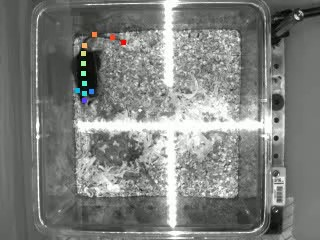
\includegraphics[width=\textwidth]{figures/deeplabcut-top-example-4128-2020-12-02-1-00-37.jpg}
    \caption{}
    \label{fig:deeplabcut-top-example}
  \end{subfigure}
  \begin{subfigure}{0.45\textwidth}
    \centering
    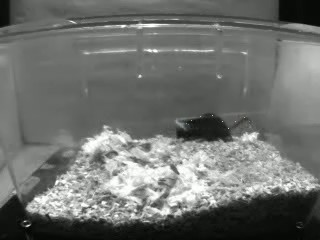
\includegraphics[width=\textwidth]{figures/deeplabcut-lateral-example-4128-2020-12-02-1-00-37.jpg}
    \caption{}
    \label{fig:deeplabcut-lateral-example}
  \end{subfigure}
  \caption[Salida de DeepLabCut.]
  {Salida de DeepLabCut del animal 4128 el 02-12-2020, 1:00:37. \ref{fig:deeplabcut-top-example} Video de la vista cenital de la caja. Los puntos sobre el animal son los dibujados por DeepCutLab para rastrear las partes del animal. \ref{fig:deeplabcut-lateral-example} Video de la vista lateral de la caja.}
  \label{fig:deeplabcut-outputexamples}
\end{figure}

\begin{table}[h]
  \centering
  \begin{tabular}{|c|c|c|c|c|c|c|}
  \hline
    & Nosex & Nosey & Noselikelihood & Headx & Heady & ... \\
  \hline
  0 & 136.165344 & 177.722496 & 0.000084 & 129.790253 & 174.772552 & ... \\
  1 & 162.032005 & 201.444756 & 0.942181 & 168.152061 & 202.420639 & ... \\
  2 & 156.297043 & 200.326378 & 0.000073 & 162.436028 & 203.156837 & ... \\
  3 & 155.370415 & 199.043297 & 0.000277 & 159.507599 & 200.199928 & ... \\
  4 & 149.272644 & 197.677170 & 0.000045 & 155.493912 & 198.814835 & ... \\
  ... & ... & ... & ... & ... & ... & ... \\
  \hline
  \end{tabular}
  \caption{Extracto del DataFrame de Pandas de los datos sin procesar de DeepLabCut.}
  \label{tab:df-example}
\end{table}

% Triangulations
\begin{figure}[H]
  \centering
  \begin{subfigure}{0.45\textwidth}
    \centering
    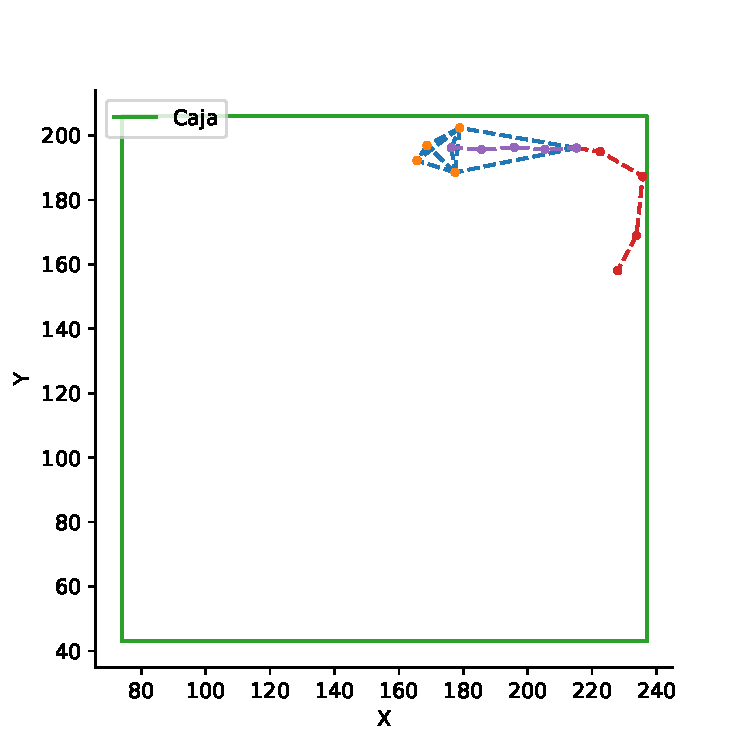
\includegraphics[width=\textwidth]{figures/triangulation-top-4128-2020-12-02.pdf}
    \caption{Vista cenital.}
  \end{subfigure}
  \begin{subfigure}{0.45\textwidth}
    \centering
    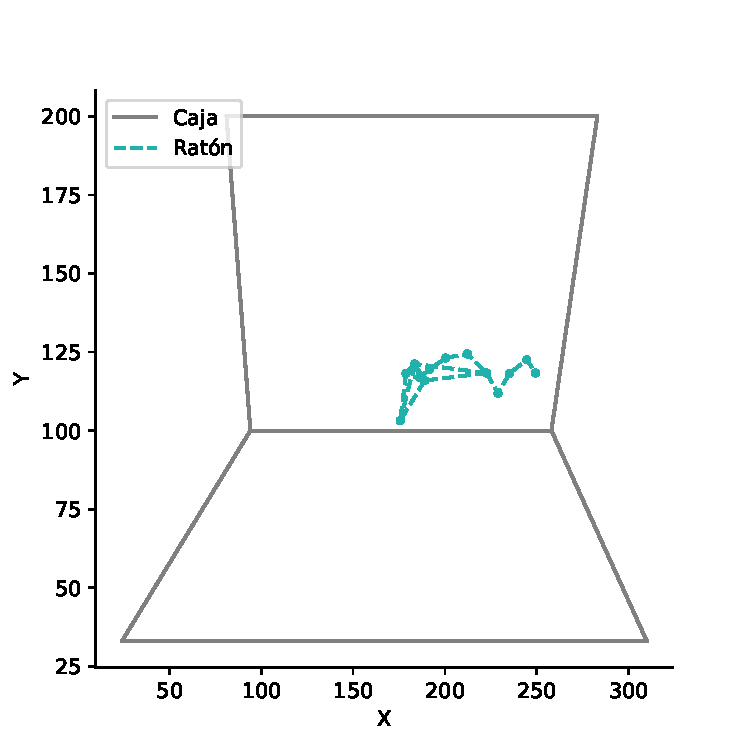
\includegraphics[width=\textwidth]{figures/triangulation-lateral-4128-2020-12-02.pdf}
    \caption{Vista lateral.}
  \end{subfigure}
  \caption{Triangulaciones de los puntos del animal 4128 el 02-12-2020, 1:00:37.}
  \label{fig:triangulations}
\end{figure}

\subsection{Filtrado e interpolación}

% Raw trayectory
\begin{figure}[H]
  \centering
  \begin{subfigure}{0.45\textwidth}
    \centering
    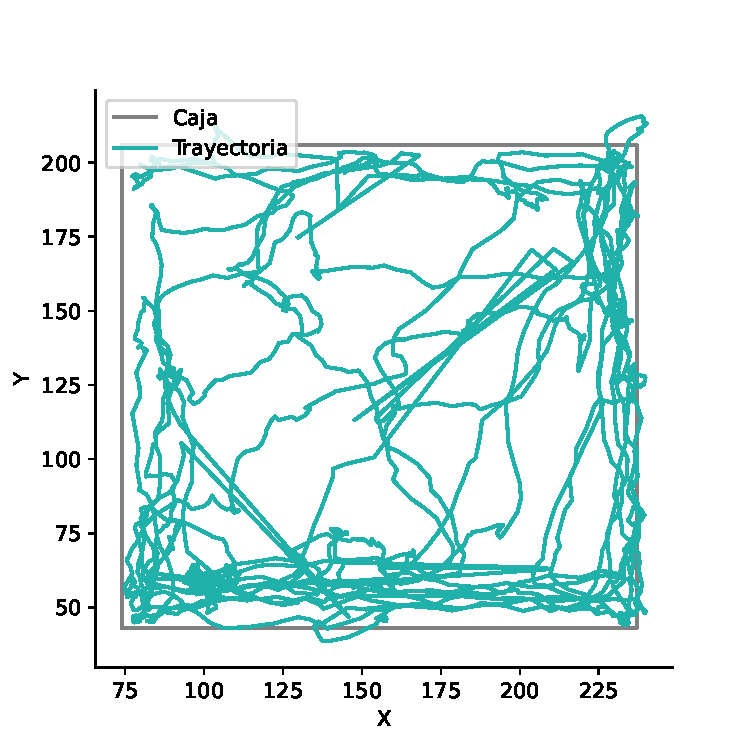
\includegraphics[width=\textwidth]{figures/raw-trayectory-top-4128-2020-12-02.pdf}
    \caption{Vista cenital.}
  \end{subfigure}
  \begin{subfigure}{0.45\textwidth}
    \centering
    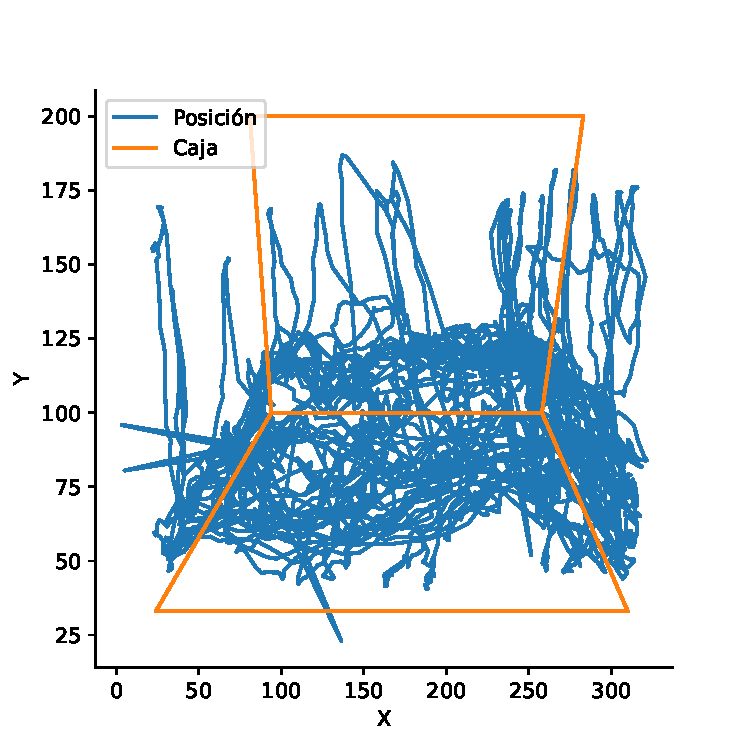
\includegraphics[width=\textwidth]{figures/raw-trayectory-lateral-4128-2020-12-02.pdf}
    \caption{Vista lateral.}
  \end{subfigure}
  \caption{Trayectoria de un punto de cabeza del animal 4128 el 02-12-2020.}
  \label{fig:raw-trayectories}
\end{figure}

% Filtered trayectory
\begin{figure}[H]
  \centering
  \begin{subfigure}{0.45\textwidth}
    \centering
    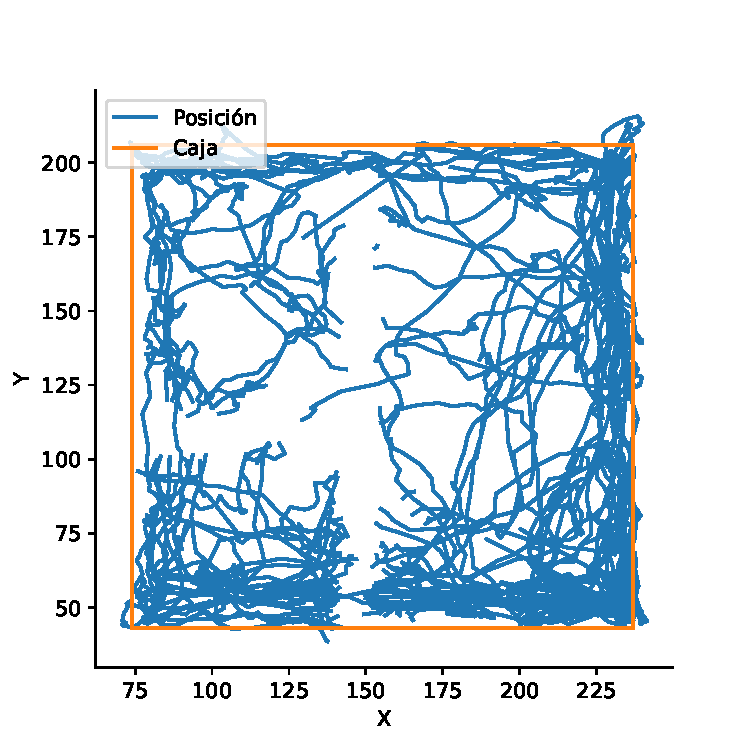
\includegraphics[width=\textwidth]{figures/filtered-trayectory-top-4128-2020-12-02.pdf}
    \caption{Vista cenital.}
  \end{subfigure}
  \begin{subfigure}{0.45\textwidth}
    \centering
    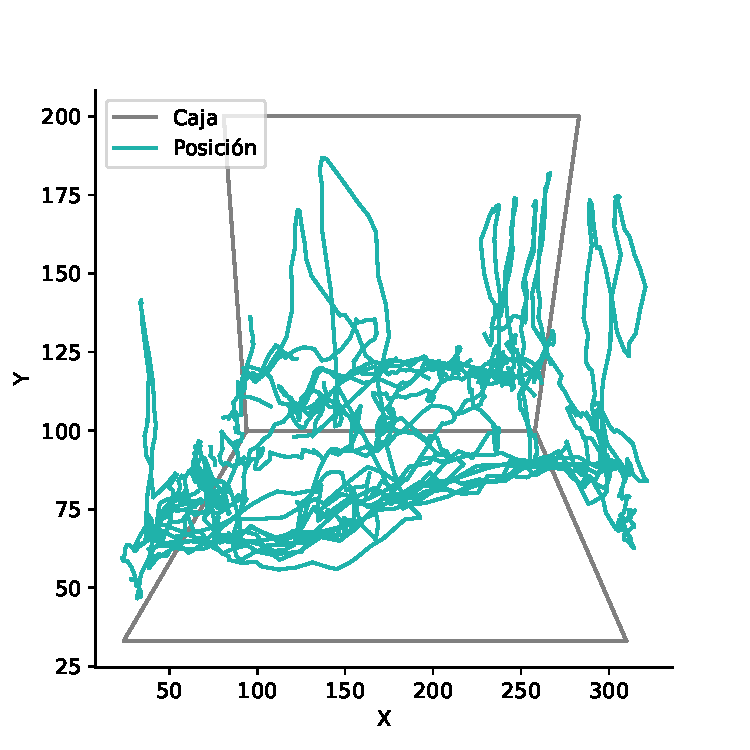
\includegraphics[width=\textwidth]{figures/filtered-trayectory-lateral-4128-2020-12-02.pdf}
    \caption{Vista lateral.}
  \end{subfigure}
  \caption{Trayectoria filtrada de un punto de la cabeza del animal.}
  \label{fig:filtered-trayectories}
\end{figure}

% Interpolated trayectory
\begin{figure}[H]
  \centering
  \begin{subfigure}{0.45\textwidth}
    \centering
    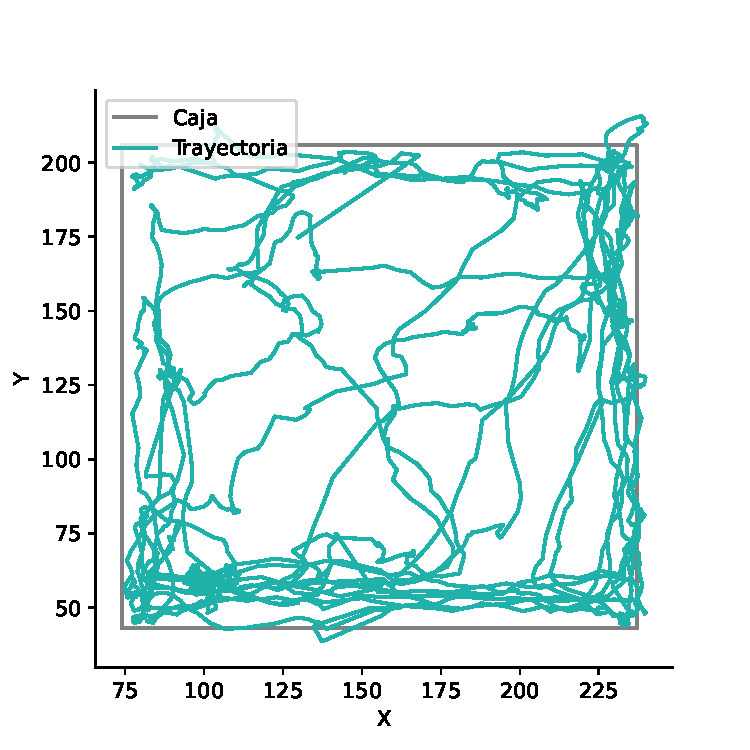
\includegraphics[width=\textwidth]{figures/interpolated-trayectory-top-4128-2020-12-02.pdf}
    \caption{Vista cenital.}
  \end{subfigure}
  \begin{subfigure}{0.45\textwidth}
    \centering
    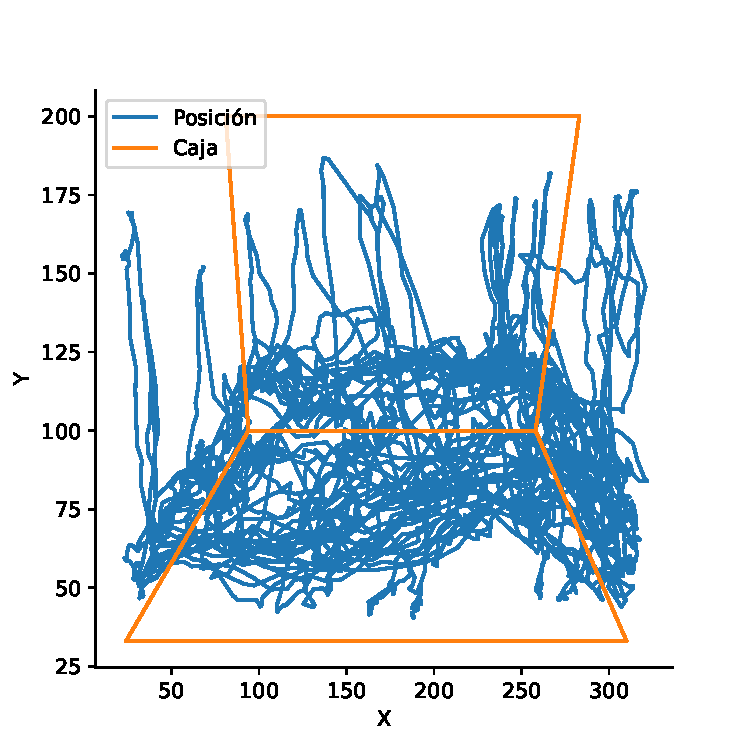
\includegraphics[width=\textwidth]{figures/interpolated-trayectory-lateral-4128-2020-12-02.pdf}
    \caption{Vista lateral.}
  \end{subfigure}
  \caption{Trayectoria interpolada de un punto de la cabeza del animal.}
  \label{fig:interpolated-trayectories}
\end{figure}


\subsection{Computo de variables a analizar}

\newpage
\section{Procesado de datos}

\subsection{Matriz de similitud}

\subsection{Agrupamiento por afinidad}

\subsection{Reducción de dimensionalidad para visualización}

\subsection{Entrenamiento de una red neuronal}


% \section{Pruebas \LaTeX}
% \subsection{Código}
% 
% \begin{mypython}[caption={Titulo del algoritmo/código.},label={alg:etiqueta}]
% def sum_list_limits_1(a, lower, upper):
%     if lower > upper:
%         return 0
%     else:
%         return a[upper] + sum_list_limits_1(a, lower, upper - 1)
% \end{mypython}
% 
% El código~\ref{alg:etiqueta} es un ejemplo en Python.
% 
% 
% 
% \begin{algorithm}[H]
% \begin{algorithmic}[1]
% \STATE $\forall i \in V$, \ let $i$ be an isolated community
% \STATE $o=permutation(V)$
% \FOR{$k \ \in \ o$}
% \STATE search in $A$ all the neighbours of $k$, $j$
% \STATE $\forall j$, calculate $\Delta Q_k(j)$ in matrix $\mathcal{M}$
% \STATE $j^*=\{ \ j \ | \ \Delta Q_k(j^*)=\max_j\{Q_k(j)\} \ \}$
% \IF{$\Delta Q_k(j^*)>0$}
% \STATE{Move node $k$ to $j^*$ 's community}
% \ELSE
% \STATE{$k$ remains in its community}
% \ENDIF
% \ENDFOR
% \end{algorithmic}\caption{\textit{Additional Louvain} \textbf{input}=$\left(A, \ \mathcal{M}\right)$ \textbf{output}=$P$}
% \label{alg:AdditionalLouvain}
% \end{algorithm}
% 
% En el algoritmo~\ref{alg:AdditionalLouvain} aparece un ejemplo en pseudocódigo.
En esta sección se describe los resultados obtenidos en el TFG, en caso de realizar propuestas para su resolución. Puede sustituirse por ejemplos u omitirse.


\chapter{Conclusiones}
En este capítulo se detallan las conclusiones derivadas del TFG y la propuesta de posibles trabajos futuros.

Las citas del texto Autor \cite{giaquinta}, Autor \cite{fortune}, Autor \cite{fortuneB}, Autor \cite{mitchell} y Autor \cite{morrey} deben ir referenciadas en la bibliografia.


\section{Texto de relleno}

\lipsum[1-18]



%%%%%%%%%%%%%%%%%%%%%%%%%%%%%%% Bibliografía %%%%%%%%%%%%%%%%%%%%%%%%%%%%%%%

\phantomsection
\addcontentsline{toc}{chapter}{Bibliografía}

\footnotesize{
%\bibliographystyle{hispa}
\bibliographystyle{IEEEtran}
\bibliography{bibliografia}
}



% No expandir elementos para llenar toda la página
\raggedbottom
\afterpage{\blankpage}

\newpage




%%%%%%%%%%%%%%%%%%%%%%%%%%%%%%% Apéndices %%%%%%%%%%%%%%%%%%%%%%%%%%%%%%%

\appendix

\phantomsection
\addcontentsline{toc}{chapter}{Apéndices}

\mbox{}
\vfill
\begin{center}
\begin{Huge}
\textbf{Apéndices}
\end{Huge}
\end{center}
\vfill
\mbox{}
\thispagestyle{empty}

\newpage
\mbox{}
\thispagestyle{empty}
\newpage


% Primer apéndice
\chapter{Apéndice 1}
\label{sec:apendice}
\section{Salida de la validación cruzada de la red convolucional.}

\begin{verbatim}
    Fold 1
    -------
    Epoch 1, Training loss 0.6996589693529852
    Epoch 10, Training loss 0.3914181091662111
    Epoch 20, Training loss 0.028187466969970484
    Epoch 30, Training loss 0.006742463795061426
    Epoch 40, Training loss 0.003754144479271731
    Epoch 50, Training loss 0.002467109620895293
    Epoch 60, Training loss 0.0018386000028265531
    Epoch 70, Training loss 0.0014798810073537833
    Epoch 80, Training loss 0.001202181870766431
    Epoch 90, Training loss 0.0010188377396927494
    Epoch 100, Training loss 0.0009259502981124036
    Accuracy train: 100.0%
    Accuracy val: 53.84615384615385%
    
    Fold 2
    -------
    Epoch 1, Training loss 0.6590047591719134
    Epoch 10, Training loss 0.3379397751099762
    Epoch 20, Training loss 0.02254703572025287
    Epoch 30, Training loss 0.006650687512826581
    Epoch 40, Training loss 0.003737638848659786
    Epoch 50, Training loss 0.0025370304577116824
    Epoch 60, Training loss 0.0019184314137680627
    Epoch 70, Training loss 0.00152091032581164
    Epoch 80, Training loss 0.0012658066058567532
    Epoch 90, Training loss 0.0010788602454737685
    Epoch 100, Training loss 0.00092578063789727
    Accuracy train: 100.0%
    Accuracy val: 60.0%
    
    Fold 3
    -------
    Epoch 1, Training loss 0.667039497145291
    Epoch 10, Training loss 0.4190175721700164
    Epoch 20, Training loss 0.04101331377851552
    Epoch 30, Training loss 0.010446132586910337
    Epoch 40, Training loss 0.005377942471411721
    Epoch 50, Training loss 0.003532323196139615
    Epoch 60, Training loss 0.0026109476099406294
    Epoch 70, Training loss 0.002050086105544784
    Epoch 80, Training loss 0.0016736525467840485
    Epoch 90, Training loss 0.0014004294222187995
    Epoch 100, Training loss 0.0011978454296758141
    Accuracy train: 100.0%
    Accuracy val: 64.61538461538461%
    
    Fold 4
    -------
    Epoch 1, Training loss 0.6882521503273098
    Epoch 10, Training loss 0.31157968178305817
    Epoch 20, Training loss 0.017680644784617804
    Epoch 30, Training loss 0.005089276510554409
    Epoch 40, Training loss 0.0028648498048604435
    Epoch 50, Training loss 0.001965091866612516
    Epoch 60, Training loss 0.001495680903320752
    Epoch 70, Training loss 0.001185416783666641
    Epoch 80, Training loss 0.0010830991498018004
    Epoch 90, Training loss 0.0008304081024232738
    Epoch 100, Training loss 0.0007286544534466905
    Accuracy train: 100.0%
    Accuracy val: 60.0%
    
    Fold 5
    -------
    Epoch 1, Training loss 0.6766076351719341
    Epoch 10, Training loss 0.2829631914909201
    Epoch 20, Training loss 0.04570655433605585
    Epoch 30, Training loss 0.005027402004015621
    Epoch 40, Training loss 0.0028682147691644535
    Epoch 50, Training loss 0.0019647855254428075
    Epoch 60, Training loss 0.0014853175453444938
    Epoch 70, Training loss 0.0011834773458863257
    Epoch 80, Training loss 0.0009805411278523087
    Epoch 90, Training loss 0.0008358971513346126
    Epoch 100, Training loss 0.0007206922087663833
    Accuracy train: 100.0%
    Accuracy val: 57.8125%
    
    All folds completed!
    Mean accuracy: 59.25480769230769%
    \end{verbatim}

% Fin del documento
\end{document}
